\subsubsection{Implementation}
Adapting the trivial iterative implementation of the FFT to use cilk \textbf{effectively} proved to be a harder task than the adoption of the recursive implementation. 

The first thing we tried was to extract the innermost loop to its own function, use cilk\_spawn in the middle loop to call these functions and then cilk\_sync after the middle loop, as follows: 

Extracted list listing:
\begin{lstlisting}
  void loop_helper(double complex *in, double complex *out, int len, int k, int i)
  {
   double complex omega = cexp(-2*k*PI*I/i);
   for(int j = 0; j < len/i; j++) {
       double complex twiddle = omega * out[j*i + k + i/2];
       out[j*i + k + i/2] = out[j*i + k] - twiddle;
       out[j*i + k] = out[j*i + k] + twiddle;
   }
  }
\end{lstlisting}

Call: 
\begin{lstlisting}
 for(int k = 0; k < i/2; k++) {  
           cilk_spawn loop_helper(in, out, len, k, i);
         }
         cilk_sync;
\end{lstlisting}

This implementation did however not lead to any improvement in execution time (sometimes it was even slower than the sequential implementation). Using the cutoff strategy here did also not help much. 

This lead to our second and more complex solution, which utilizes a divide and conquer approach. We divide the iteration space of the middle loop in half and tell the cilk runtime that both halfes can be executed in parallel. To avoid creating too many tasks, we also implementent a cutoff after which the execution will be continued sequentially. The principle of the implementation is as follows: 

Loop divide and conquer: 
\begin{lstlisting}
void loop_helper_dq(double complex *in, double complex *out, int len, int i, int from, int to)
{
  if((to - from) <= 64) {
    ... //under cutoff continue sequentially
  }
  else {
    cilk_spawn loop_helper_dq(in, out, len, i, from, from + (to - from)/2);
    cilk_spawn loop_helper_dq(in, out, len, i, from + (to - from)/2, to);
  }
}
\end{lstlisting}

Calling code (spawning the loop_helper_dg function here is the equivalent of the k-loop in the other iterative implementations)
\begin{lstlisting}
	cilk_spawn loop_helper_dq(in, out, len, i, 0, i/2);
    cilk_sync;
\end{lstlisting}

While this is now again a recursive implementation, it still works according to the same principle as the original iterative implementation. 

\subsubsection{Performance}

Average speedup:

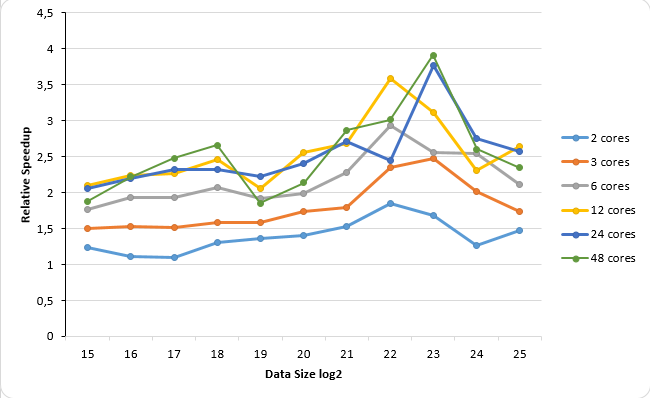
\includegraphics[width=\textwidth]{cilk_it_avg.png}

Best observered speedup:

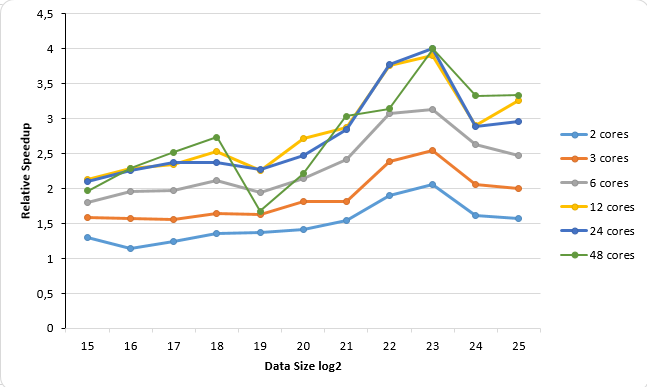
\includegraphics[width=\textwidth]{cilk_it_best.png}

The graphs again show the same pattern of the speedup scaling with the ammount of data supplied. 

While the further above mentioned optimizations of the implementation lead to some speedup, this implementation is still the implementation with the lowest overall speedup. We believe the reason for this is that cilk is not optimized for dealing with an implimitation that follows the principle of an iterative implementation. Another reason for the low speedup is the same problem with the cpu usage that has already been encountered by the recursive implementation.